\begin{document}
\subsection{Semantische Analyse/Optimierung}

\begin{frame}{Semantische Analyse}
	\begin{itemize}
		\item PP beschäftigt sich (bis auf Typinferenz) nur kurz mit semantischer Analyse
		\item Typchecks/-inferenz, Namensanalyse
		\item $\leadsto$ weiterführende (Master-)Vorlesungen am IPD
	\end{itemize}
\end{frame}

\begin{frame}{Optimierung}
  \begin{itemize}
    \item Moderne Compiler haben i.d.R. (mindestens) eine Zwischensprache, bspw.
    \begin{itemize}
      \item GCC: Generic, GIMPLE, RTL
      \item LLVM, libFirm
      \item GHC: Core, STG
    \end{itemize}
    \item Vorteil: Optimierungen müssen nur einmal implementiert werden
  \end{itemize}
\end{frame}

\subsection{Zwei Beispiele}

\begin{frame}{Beispiel: GCC}
  \begin{figure}
    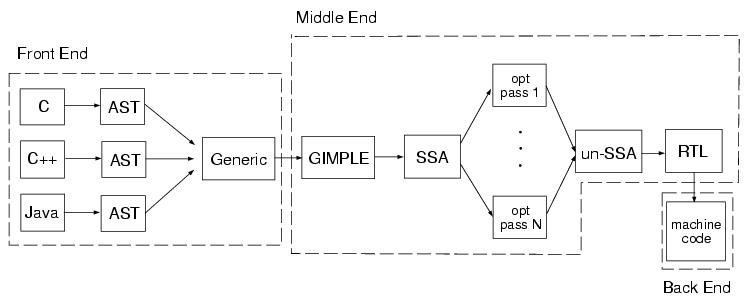
\includegraphics[width=\textwidth]{images/gcc.jpg}
  \end{figure}

  \begin{itemize}
    \item Generic: Sprachunabhängiger Output des Frontend
    \item GIMPLE: Für Optimierungen (SSA: Spezielle Form)
    \item RTL: Für Registerallokation, Instruktionsauswahl
    \item Ca. 15 Mio. Zeilen Code (2019, laut Wikipedia)
  \end{itemize}
\end{frame}

\begin{frame}{Beispiel: GHC}
  \begin{figure}
    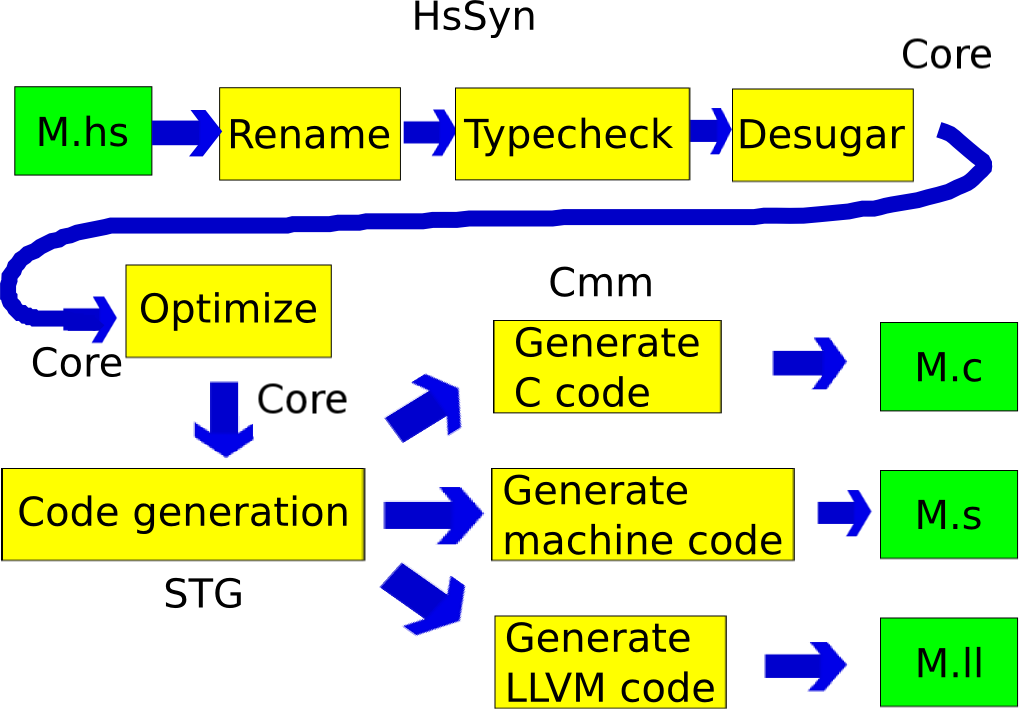
\includegraphics[width=0.6\textwidth]{images/ghc.png}
  \end{figure}

  \begin{itemize}
    \item Core: \enquote{$\lambda$-Kalkül mit Extras}, für Optimierungen
    \item STG: Spineless Tagless Graph-Machine, für Codeerzeugung
    \item Cmm: \enquote{C minus minus}, für Codeerzeugung
    \item Ca. 600.000 Zeilen Code, $\frac{3}{4}$ davon Haskell (selbst gezählt)
  \end{itemize}
\end{frame}

\section{propalang}

\begin{frame}{propalang}
  \code{code/propalang.pp}

  \begin{itemize}
    \item \href{https://pbrinkmeier.de/propalang.zip}{pbrinkmeier.de/propalang.zip}
    \item Im Repository: demos/java/propalang
    \item Parser für Expressions und Statements
    \item Interpreter: \texttt{java Main -- run test.pp}
  \end{itemize}
\end{frame}

\begin{frame}{propalang: Aufgaben}
  \code{code/propalang.pp}

  \begin{itemize}
    \item Erweitert den Parser um eine Divisionsoperation \texttt{/}
    \begin{itemize}
      \item \texttt{new OperatorExpression(Operator.DIVIDE, ...)}
    \end{itemize}
    \pause
    \item Erweitert den Parser um Schleifen \texttt{while} und \texttt{for}
    \begin{itemize}
      \item \texttt{while (condition) loopStmt;}
      \item \texttt{for (init; condition; post) loopStmt;}
      \item \texttt{new WhileStatement(...)}
      \item Keine neue AST-Klasse für \texttt{for}!
    \end{itemize}
  \end{itemize}
\end{frame}

\section{Ende}

\begin{frame}{Letzte Folie}
  \begin{itemize}
    \item Morgen, Mi, 09.02. um 14:00: Letzte Vorlesung
    \item ÜB-Korrekturen: Bis spätestens Ende Februar
    \item Klausur: 08.04.2022, 12:00
    \item Tutoriumsfolien, -code, etc.: \href{https://github.com/pbrinkmeier/pp-tut}{github.com/pbrinkmeier/pp-tut}
    \item Fragen auch gerne an \texttt{pp-tut@pbrinkmeier.de} :)
  \end{itemize}

  \vfill

  Danke fürs Kommen und eine gute Prüfungsphase!
\end{frame}
\end{document}